\documentclass[10pt,a4paper]{article}

% ---------- Packages ----------
\usepackage[utf8]{inputenc}
\usepackage[T1]{fontenc}
\usepackage[english]{babel}
\usepackage{microtype}
\usepackage[a4paper,margin=2.4cm]{geometry}
\usepackage{lmodern}
\usepackage{amsmath, amssymb}
\usepackage{graphicx}
\usepackage{booktabs}
\usepackage{array}
\usepackage{multirow}
\usepackage{tabularx}
\usepackage{caption}
\usepackage{subcaption}
\usepackage[table]{xcolor}
\usepackage{listings}
\usepackage[hidelinks]{hyperref}
\usepackage{enumitem}
\usepackage{fancyvrb}
\usepackage{titlesec}
\usepackage[round,authoryear]{natbib}

% ---------- Style ----------
\titleformat*{\section}{\large\bfseries}
\titleformat*{\subsection}{\normalsize\bfseries}
\setlength{\parskip}{0.4em}
\setlength{\parindent}{0em}
\emergencystretch=1.5em

\definecolor{kwcolor}{RGB}{0,80,160}
\definecolor{strcolor}{RGB}{160,0,0}
\definecolor{cmtcolor}{RGB}{0,120,0}
\lstdefinestyle{plain}{
  basicstyle=\ttfamily\footnotesize,
  keywordstyle=\color{kwcolor},
  stringstyle=\color{strcolor},
  commentstyle=\color{cmtcolor}\itshape,
  showstringspaces=false,
  breaklines=true,
  frame=single,
  framerule=0.3pt,
  rulecolor=\color{gray!50},
  language=Python,
  numbers=none,
  xleftmargin=0.5em,
  xrightmargin=0.5em
}
\lstset{style=plain}

% ---------- Title ----------
\title{\textbf{Summarising Football Match Commentaries:\\
A Comparative Study of Prompting and Fine-tuning\\
on Long-form Sports Audio Transcripts}}
\author{Marco Panciera \quad Christian Dalfarra\\
\small Applied Natural Language Processing\\
\small University of Trento}
\date{May 2026}

% ============================================================
\begin{document}
\maketitle

% ---------- Abstract ----------
\begin{abstract}
We study automatic summarisation of long football-match commentaries, where the input is a Whisper transcription of $\sim$2.5 hours of live BBC radio audio (mean $\sim$25\,000 words) and the target is a $\sim$200-word match report. We construct a custom dataset of 99 matches spanning 1983--2026 and 12 competition/stage categories, with summaries generated by prompting search-enabled GPT-4 on a per-match basis --- grounded in web-retrieved match reports rather than the transcript --- and used as references during both training and evaluation.

We compare two orthogonal design axes: \emph{input handling} (chunk-and-aggregate vs.\ long-context with LED-16384) and \emph{learning paradigm} (zero/few/CoT prompting vs.\ supervised fine-tuning) across three architectures (FLAN-T5-Large, BART-Large-CNN, LED-base). Both fine-tuned pipelines reach ROUGE-L $\approx 0.248$ (LED long-context $0.248$, BART chunk-merger $0.248$), a $+55\%$ relative improvement over the strongest prompting baseline; paired bootstrap tests confirm the fine-tuning-vs-prompting gap is significant at $n=9$ while the gap between the two fine-tuned pipelines is not. Null baselines temper that headline: another match's reference --- correct format, every fact wrong --- already scores ROUGE-L 0.208, and a generic template containing no match-specific content outscores every prompting condition, so the margin that survives a format-matched control is $+0.040$ ROUGE-L (CI $[+0.022, +0.059]$). We further document a costly empty-reference dataset bug that masked the true performance ceiling by a factor of $\sim$1.8$\times$. Rule-based faithfulness probes and NLI entailment against the source then show where the reference-based metrics stop tracking accuracy. Across all eleven conditions the two agree loosely and positively (Spearman $\rho = +0.41$ to $+0.63$ on the team-mention, scoreline, scorer and NLI probes), but the relationship collapses at the top of the leaderboard, exactly where a metric is used to choose a model: fine-tuned LED --- which leads on \emph{every} reference-based metric --- achieves only 2/9 correct scorelines and 2\% NLI-supported sentences, and fine-tuned BART states the correct final score in 0 of 9 matches with zero sentences entailed by the transcript. The best-grounded conditions are the transcript-copying prompted baselines that both fine-tuned models outrank on ROUGE.
\end{abstract}

% ============================================================
\section{Introduction}

Automatic summarisation of long-form spoken-language transcripts is a stress test for modern sequence-to-sequence models: inputs routinely exceed the context window of a standard transformer, outputs require selective abstraction over hours of fragmented commentary, and references for training data are scarce. Football match commentaries are an especially appealing test bed because (i)~the input is structurally noisy (live audio, overlapping speakers, prosodic emphasis on irrelevant detail), yet (ii)~the desired output --- a match report --- has a stable, learnable surface format.

This project asks two narrowly-scoped, empirically answerable questions:

\begin{enumerate}[leftmargin=*,itemsep=2pt,topsep=2pt]
\item Given a $\sim$25\,000-word transcript and an output budget of $\sim$200 words, is it better to \emph{chunk and aggregate} or to use a \emph{long-context} encoder?
\item For each input strategy, does \emph{supervised fine-tuning} on a small in-domain dataset outperform \emph{prompting} of a general-purpose model?
\end{enumerate}

We instantiate the cross product on three architectures (FLAN-T5-Large, BART-Large-CNN, LED-base-16384) and three prompting strategies (zero-shot, few-shot, chain-of-thought \citep{wei2022cot}), giving eleven evaluated conditions (nine prompting, two fine-tuned) on a held-out 9-match test set. Ten of these are distinct: the few-shot long-context cell fell back to its zero-shot variant through an implementation gap we disclose in Section~\ref{sec:results}.

\paragraph{Contributions.}
\begin{itemize}[leftmargin=*,itemsep=2pt,topsep=2pt]
\item A custom 99-match dataset (BBC radio audio $\to$ Whisper transcript $\to$ GPT-4 reference summary), built end-to-end for this project.
\item A \emph{chunk-merger} fine-tuning recipe for BART in which the training input is the concatenation of pre-trained per-chunk summaries, eliminating the train/inference distribution mismatch of naive truncated-input training and improving ROUGE-L by $+69\%$ over the same pre-trained model. A clean-trained LED long-context fine-tune matches this pipeline (0.248 vs.\ 0.248), confirming that at $N=80$ neither architecture holds a decisive advantage.
\item A systematic comparison of prompting vs.\ fine-tuning across two input pipelines, with bootstrap confidence intervals and rule-based faithfulness probes that locate where ROUGE stops tracking factual accuracy: the two correlate weakly but positively across the condition range, and come apart at the top of it, where the ROUGE-best model never states the correct final score.
\item Null baselines that bound how much of the reported overlap is template imitation: a wrong match's reference reaches 84\% of our best model's ROUGE-L, and every prompting condition scores below a content-free template --- so reference-based gaps on this dataset must be read against a format floor rather than against zero.
\item A documented engineering history of five distinct silent failures encountered during LED fine-tuning, of independent practical value for small-scale long-document fine-tuning.
\end{itemize}

% ============================================================
\section{Related Work}

\paragraph{Long-document summarisation.}
Standard transformer summarisers (BART \citep{lewis2020bart}, PEGASUS \citep{zhang2020pegasus}, T5 \citep{raffel2020t5}) cap input at 1024 tokens, far below the $\sim$30\,000-token regime of full-match transcripts. Two families of solutions have emerged: (i) extend the attention mechanism to support longer contexts (Longformer / LED \citep{beltagy2020longformer}); (ii) chunk the document, summarise each piece, and recombine \citep{see2017pointer}. We compare both directly on the same data.

\paragraph{Prompting vs.\ fine-tuning.}
Instruction-tuned models (FLAN-T5 \citep{chung2022flan}, GPT-style models \citep{brown2020gpt3}) can perform many summarisation tasks zero-shot. Fine-tuning on small in-domain data, however, often outperforms prompting when the target distribution differs systematically from web-scale pre-training data. Sports commentary is one such case: pre-training corpora contain match reports as \emph{outputs} but rarely raw radio transcripts as inputs.

\paragraph{Faithfulness.}
\citet{maynez2020faithfulness} document that abstractive summarisers routinely introduce content not entailed by the source. ROUGE \citep{lin2004rouge} cannot detect this; BERTScore \citep{zhang2020bertscore} captures semantic but not factual correctness. We provide qualitative evidence of hallucination in our trained models and discuss this limitation in Section~\ref{sec:limitations}.

% ============================================================
\section{Dataset Construction}
\label{sec:dataset}

\subsection{Source selection and audio collection}
We selected 100 football matches\footnote{One audio file failed extraction and was dropped, leaving 99 usable matches.} from the publicly-available BBC Radio 5 Live archive on YouTube, spanning 43 years (1983--2026) and 12 competition/stage categories (finals and qualifiers counted separately): World Cup (32), UEFA Champions League (17), Premier League (15), Euros (14), UCL final (8), WC qualifiers (5), FA Cup (2), Nations League (2), UEFA League Final, Euro final, WC final, UECL final (1 each). The mix is England-heavy --- most fixtures involve a home-nations team, reflecting the source --- with a deliberate inclusion of neutral fixtures (Spain--Germany, Argentina--Poland) to test out-of-distribution generalisation. Matches were downloaded as MP3 via \texttt{yt-dlp}, totalling $\sim$19~GB of audio.

\subsection{Speech-to-text transcription}
Each MP3 was processed by OpenAI Whisper \texttt{small} \citep{radford2023whisper}. For every Whisper segment, we additionally extracted per-segment prosodic features --- mean pitch (Hz) and RMS energy --- using \texttt{librosa}. Each match produces three artefacts:

\begin{itemize}[leftmargin=*,itemsep=2pt,topsep=2pt]
\item \texttt{\{id\}\_transcript.txt} --- the full, unsegmented commentary (mean 130~KB, $\sim$25\,000 words).
\item \texttt{\{id\}\_segments.txt} --- the same text split into time-aligned Whisper utterances with pitch and energy annotations.
\item \texttt{\{id\}.json} --- structured token-level alignment.
\end{itemize}

A representative segment line:
\begin{quote}
\small\ttfamily
[0.00 - 6.80] P:1767.91 E:0.031 | Wenger's Arsenal look like this, Seaman in goal, a back four of Dixon, Keown, Adams and Cole.
\end{quote}

Whisper transcription introduces systematic errors on player names (``Bergkamp'' $\to$ ``Burgkamp'', ``Wenger's'' $\to$ ``Vengas'') that propagate through every downstream pipeline and bound the achievable surface-token overlap from above.

\subsection{Reference summary generation}
\label{sec:gpt_targets}
The dataset has no naturally-paired ground-truth summaries for radio commentary. We therefore generated reference summaries by prompting GPT-4 \citep{openai2023gpt4} on a per-match basis via the ChatGPT web interface with search enabled: for each match the model was given the match identifier (year, competition, teams) and instructed to retrieve contemporary accounts of the fixture before writing a structured summary. We manually checked the citations returned for every match and confirmed that each report drew on the BBC website among its sources. Grounding generation in retrieved sources anchors the factual content (scores, scorers, key events) in published accounts rather than the model's parametric memory. The output template is fixed:

\begin{quote}
\small\itshape
Line 1: \{TeamA\} \{scoreA\}--\{scoreB\} \{TeamB\}\\
Line 2: \{Competition\}, \{Stadium\}, \{City\} -- \{Date\}\\
Lines 3+: 2--4 paragraph report covering result, key events, and a brief tactical note.\\
Final block: bullet list of key events (e.g.\ ``27' -- Gordon Smith goal'').
\end{quote}

Mean reference length is $\sim$1.2~KB ($\sim$190 words; range 100--365).

\paragraph{Methodological note.}
Using a large language model to generate references introduces an evaluation bias even with retrieval: the references reflect web-sourced match reports as filtered and rewritten by GPT-4 at generation time, and they remain \emph{ungrounded in the transcript} our models actually read --- events a radio commentator dwells on may be absent from a written report and vice versa. Retrieval also weakens reproducibility: search results change over time, so regenerating the references would not yield byte-identical targets. We discuss this candidly in Section~\ref{sec:limitations}. The alternative --- human-written summaries for 99 matches --- was outside the scope of a course project. References were spot-checked manually and accepted as a working approximation.

\subsection{Splits and statistics}
A stratified train/val/test split of 80/10/9 was generated once (\texttt{scripts/generate\_splits.py}) and committed to the repository to ensure reproducibility. Test matches deliberately span eras and competitions (1983 FA Cup, 2001 FA Cup, 2019 UCL Final, 2021/2022/2024 internationals, 2026 UCL group stage). Dataset statistics are summarised in Table~\ref{tab:dataset}.

\begin{table}[h]
\centering\small
\begin{tabular}{lr}
\toprule
\textbf{Property} & \textbf{Value} \\
\midrule
Matches & 99 \\
Year coverage & 1983--2026 (43 years) \\
Competition/stage categories & 12 \\
Train / val / test & 80 / 10 / 9 \\
Mean transcript length & 130~KB ($\sim$25\,000 words) \\
Mean segments per match & $\sim$2\,100 \\
Mean reference length & 1.2~KB ($\sim$190 words) \\
Total dataset size (excl.\ raw audio) & 91~MB \\
Raw audio (gitignored) & $\sim$19~GB \\
\bottomrule
\end{tabular}
\caption{Dataset statistics for the in-project \texttt{football\_commentary\_dataset 1.0}.}
\label{tab:dataset}
\end{table}

% ============================================================
\section{Methodology}
\label{sec:method}

We compare two input-handling pipelines and two learning paradigms, giving four cells. Three architectures are evaluated where appropriate, with each prompting condition further crossed with three prompt styles (zero, few, CoT).

\subsection{Two input pipelines}

\paragraph{Chunk-and-aggregate.}
The segmented transcript is split into contiguous chunks of $\le M$ model tokens with a one-segment overlap to preserve cross-chunk context. A generator function $g(\text{chunk}) \to \text{partial summary}$ is applied to each chunk, and a merger function $m(\text{partial}_1, \dots, \text{partial}_n) \to \text{final summary}$ produces the final output. We use:
\begin{itemize}[leftmargin=*,itemsep=2pt,topsep=2pt]
\item $M = 450$ for FLAN-T5 (512-token limit minus prompt overhead),
\item $M = 900$ for BART (1024 minus output budget).
\end{itemize}
After merging, a bag-of-words cosine deduplication pass ($\ge 0.92$ similarity) removes near-duplicate \emph{adjacent} sentences from the merged output.

\paragraph{Long-context.}
The full transcript is passed to LED-base-16384 \citep{beltagy2020longformer} in a single forward pass. LED's sliding-window local attention plus full global attention on a designated BOS token make this tractable on a single T4 GPU. No chunking, no merge step.

\subsection{Prompting setup}
We test three prompt styles, fixed per model family for fair comparison:

\begin{itemize}[leftmargin=*,itemsep=2pt,topsep=2pt]
\item \textbf{Zero-shot.} An instruction (``Summarise the following football commentary into a concise match report\dots'') followed by the chunk or transcript.
\item \textbf{Few-shot.} The zero-shot prompt prefixed with two in-context (commentary $\to$ summary) examples drawn from the training set.
\item \textbf{Chain-of-thought.} A structured instruction asking the model to first enumerate goals, cards, and substitutions, then write the prose summary.
\end{itemize}

Decoding parameters are held constant across conditions: beam size 4, length penalty 1.0, no-repeat n-gram size 3, max output 256 tokens for chunk-level generation and 512 for the merge step.

\subsection{Fine-tuning setup}

\paragraph{BART chunk-merger fine-tuning.}
A naive fine-tuning recipe --- train BART on $(\text{transcript}[:1024], \text{reference})$ pairs --- exposes the model to only the first $\sim$5 minutes of a 2.5-hour match. To match the train and inference distributions, we instead train BART as the \emph{merge step} of the chunk-aggregate pipeline:

\begin{enumerate}[leftmargin=*,itemsep=2pt,topsep=2pt]
\item For each training match, run pre-trained BART-Large-CNN on every chunk to obtain $\sim$30 mini-summaries of $\sim$32 tokens each.
\item Concatenate the chunk summaries into a single $\sim$960-token intermediate.
\item Train BART to map (intermediate $\to$ reference) with a two-phase schedule: encoder frozen for 3 epochs (decoder adapts to the new target distribution), then fully unfrozen for the remainder. Early stopping on validation ROUGE-L with patience 3.
\end{enumerate}

The chunk-summary generation is cached on disk because it is the dominant one-time cost. Hyperparameters: learning rate $3\!\times\!10^{-5}$, effective batch 8 (batch 1 with gradient accumulation), \texttt{fp16}, max input 1024 tokens, max target 256 tokens.

\paragraph{LED long-context fine-tuning.}
LED-base is fine-tuned directly on (full transcript $\to$ reference) pairs, with a custom random-window sampler that, each epoch, samples a contiguous 8192-token window starting at a uniformly random offset within transcripts longer than the window. This effectively augments the training set by exposing the model to different portions of each match. Global attention is forced on the BOS token; gradient checkpointing is enabled to fit a single sequence on a T4. Hyperparameters: learning rate $2\!\times\!10^{-5}$ with a 100-step linear warm-up (earlier runs at $5\!\times\!10^{-5}$ spiked the gradient norm; see Section~\ref{sec:engineering}), batch 1 + grad-accum 8, \texttt{fp16}, max input 8192 tokens, max target 256 tokens, evaluation generation floor \texttt{min\_length=80} to expose collapse-to-empty failures (see Section~\ref{sec:engineering}).

\subsection{Evaluation}
We report ROUGE-1, ROUGE-2, and ROUGE-L F-measures (stemmed) averaged over the 9 test matches, using the \texttt{rouge\_score} package \citep{lin2004rouge}, complemented by BERTScore against the references and an NLI-based measure of grounding in the transcript (both described below). The reference-based metrics (ROUGE, BERTScore) and the source-based metrics (NLI support, faithfulness probes) deliberately measure different things; Section~\ref{sec:faith} shows they disagree sharply.

\paragraph{Bootstrap confidence intervals.}
Because $n=9$, we attach uncertainty to every aggregate: for each condition we bootstrap-resample the 9 per-match ROUGE scores (10\,000 resamples, seed 42) and report 95\% percentile intervals. To compare conditions we use a \emph{paired} bootstrap on the per-match ROUGE-L differences against the best condition, resampling matches jointly so that per-match difficulty cancels; a difference is called significant when the 95\% interval of the mean difference excludes zero.

\paragraph{Faithfulness probes.}
ROUGE cannot detect confidently-stated wrong facts, so we add two rule-based factual checks that exploit the fixed reference format (Section~\ref{sec:gpt_targets}). \emph{Score accuracy}: the reference scoreline is parsed from the reference's first line; a prediction is credited when it states the same scoreline with the correct team orientation (team-adjacent patterns such as ``\emph{Arsenal 1--2 Liverpool}'', winner-verb patterns such as ``\emph{England beat Senegal 3--0}'', and draws, which are orientation-free). \emph{Scorer recall}: scorer names are parsed from the reference's key-events block; we measure the fraction mentioned in the prediction, matching surnames case- and accent-insensitively with a fuzzy threshold (\texttt{SequenceMatcher} ratio $\ge 0.85$) to tolerate Whisper misspellings. We also report a weaker sanity check, whether \emph{both team names} appear at all. \emph{Named-entity precision}: because scorer recall is blind to over-generation (a summary naming ten players, one correct, still scores well), we extract \texttt{PERSON} entities from each prediction with spaCy and measure the fraction whose surname matches a person in the reference (its scorers plus any \texttt{PERSON} in the report, same fuzzy threshold); we report it alongside the mean number of distinct people named, since precision is only meaningful when that count is not near zero. Extraction code is \texttt{report/compute\_analysis.py}; per-match extractions were audited manually.

\paragraph{Null baselines.}
Because the references follow a fixed template (Section~\ref{sec:gpt_targets}), a model can score on surface-overlap metrics through format imitation alone. To bound that effect we score five ``predictions'' that contain no correct information about the match they are evaluated against (code \texttt{report/compute\_nullbaselines.py}): another \emph{test} match's reference (averaged over all eight donors), a random \emph{training} reference (20 donors), a hand-written generic match report with and without the real team names substituted in, and --- as the standard extractive control --- the lead 190 words of the transcript, length-matched to the mean reference. All use the identical stemmed \texttt{rouge\_score} configuration and the same 9 test matches, and we compare the best model against the strongest null with the same paired bootstrap.

\paragraph{Semantic metrics.}
Two further metrics were computed locally, post-hoc, on the saved predictions (code \texttt{report/compute\_semantic.py}). \emph{BERTScore} \citep{zhang2020bertscore} F1 (RoBERTa-large, raw scores) against the reference measures semantic similarity to the target beyond n-gram overlap. \emph{NLI support rate} measures grounding in the \emph{source}: each prediction is split into sentences (long run-ons chunked at 50 words), the three most similar 60-word transcript windows are retrieved by TF-IDF, and a DeBERTa-base MNLI cross-encoder scores entailment; a sentence counts as supported when max $P(\text{entailment}) \ge 0.5$, and we report the macro-averaged supported fraction.

% ============================================================
\section{Experimental Setup}

\paragraph{Compute.} All experiments ran on free-tier Kaggle Notebooks with a single NVIDIA Tesla T4 (15.6~GB VRAM). The 12-hour-per-session and $\sim$30-GPU-hour-per-week limits dictated the experimental cadence: prompting baselines and BART fine-tuning together fit in one $\sim$2.5-hour session; LED fine-tuning is a separate $\sim$50-minute session.

\paragraph{Reproducibility.} Random seeds are fixed to 42; the train/val/test split is committed; intermediate predictions are saved to disk so the evaluation step can re-run without regenerating outputs. The dataset (excluding raw audio), code, per-run predictions, and analysis scripts are versioned in the project repository and included in the delivered archive; the audio download and transcription steps are not part of the delivered code --- the pipeline starts from the bundled transcripts --- and trained checkpoints are not included, but every reported metric is recomputable from the saved predictions.

\paragraph{Models.} Table~\ref{tab:models} summarises the architectures used.

\begin{table}[h]
\centering\small
\begin{tabular}{lllr}
\toprule
\textbf{Model} & \textbf{Role} & \textbf{Max input} & \textbf{Params} \\
\midrule
FLAN-T5-Large \citep{chung2022flan} & Prompting (chunk) & 512 & 780M \\
BART-Large-CNN \citep{lewis2020bart} & Prompting + fine-tune (chunk) & 1024 & 406M \\
LED-base-16384 \citep{beltagy2020longformer} & Prompting + fine-tune (long) & 16\,384 & 162M \\
\bottomrule
\end{tabular}
\caption{Models evaluated, by role and context-window size.}
\label{tab:models}
\end{table}

% ============================================================
\section{Results}
\label{sec:results}

\subsection{Main leaderboard}
Table~\ref{tab:main} reports ROUGE F-measures on the clean 9-match test set, with bootstrap 95\% confidence intervals on ROUGE-L. Fine-tuned LED (long-context, clean retrain) is nominally best; the paired bootstrap shows its lead over every \emph{prompting} condition is significant, while its lead over fine-tuned BART is not.

\begin{table}[h]
\centering\small
\begin{tabular}{rlrrrl}
\toprule
\textbf{Rank} & \textbf{Condition} & \textbf{R-1} & \textbf{R-2} & \textbf{R-L} & \textbf{R-L 95\% CI} \\
\midrule
1 & \textbf{finetuned\_led} (long-context)           & 0.4502 & 0.1521 & \textbf{0.2480} & [0.230, 0.266] \\
\rowcolor{gray!12} 2 & finetuned\_bart (chunk-merger, 2-phase) & 0.4205 & 0.1330 & 0.2476 & [0.208, 0.283] \\
3 & led\_long\_few$^{*}$                             & 0.2712 & 0.0531 & 0.1599 & [0.146, 0.177] \\
3 & led\_long\_zero$^{*}$                            & 0.2712 & 0.0531 & 0.1599 & [0.146, 0.177] \\
5 & led\_long\_cot$^{*}$                             & 0.2773 & 0.0559 & 0.1548 & [0.143, 0.167] \\
6 & bart\_chunk\_zero$^{*}$                          & 0.2249 & 0.0516 & 0.1467 & [0.138, 0.155] \\
7 & bart\_chunk\_cot$^{*}$                           & 0.1989 & 0.0408 & 0.1230 & [0.104, 0.142] \\
8 & bart\_chunk\_few$^{*}$                           & 0.1765 & 0.0188 & 0.1030 & [0.094, 0.113] \\
9 & flan\_chunk\_zero$^{*}$                          & 0.1164 & 0.0212 & 0.0700 & [0.054, 0.085] \\
10 & flan\_chunk\_few$^{*}$                          & 0.0770 & 0.0086 & 0.0551 & [0.045, 0.066] \\
11 & flan\_chunk\_cot$^{*}$                          & 0.0733 & 0.0148 & 0.0481 & [0.033, 0.063] \\
\bottomrule
\end{tabular}
\caption{Main results: ROUGE F-measures (stemmed) on the clean 9-match test set, with bootstrap 95\% CIs on ROUGE-L (10\,000 resamples). $^{*}$~significantly below both fine-tuned conditions (paired bootstrap CI of the ROUGE-L difference vs.\ \texttt{finetuned\_bart} excludes zero for all prompting rows; all differences are $\ge +0.08$). The fine-tuned LED--BART gap ($\Delta = -0.0004$, CI $[-0.042, +0.035]$) is \emph{not} significant. \texttt{led\_long\_few} is byte-identical to \texttt{led\_long\_zero}: an implementation fallback ran the zero-shot prompt in its place (see Observation~3).}
\label{tab:main}
\end{table}

\subsection{Null baselines: how much of ROUGE is format?}
\label{sec:null}

The references follow a fixed template: a scoreline, a competition/venue/date line, two to four paragraphs of report prose, and a bulleted key-events block. Any model that learns that template earns surface overlap before reporting a single correct fact. Table~\ref{tab:null} measures that floor directly.

\begin{table}[h]
\centering\small
\begin{tabular}{lrrr}
\toprule
\textbf{``Prediction''} & \textbf{R-1} & \textbf{R-2} & \textbf{R-L} \\
\midrule
Another \emph{test} match's reference (avg.\ over 8 donors)   & 0.3793 & 0.0952 & \textbf{0.2076} \\
A random \emph{train} match's reference (avg.\ over 20)       & 0.3533 & 0.0864 & 0.1963 \\
Generic template $+$ real team names                          & 0.3556 & 0.0680 & 0.1863 \\
Generic template, no match-specific content                   & 0.3481 & 0.0656 & 0.1758 \\
Lead-190 words of the transcript                              & 0.2624 & 0.0311 & 0.1340 \\
\midrule
\rowcolor{gray!12} \texttt{finetuned\_led} (Table~\ref{tab:main})        & 0.4502 & 0.1521 & 0.2480 \\
\texttt{led\_long\_few}, best prompting condition             & 0.2712 & 0.0531 & 0.1599 \\
\bottomrule
\end{tabular}
\caption{Null baselines. Every row above the rule contains \emph{no} correct information about the match it is scored against, except lead-190, which is verbatim source text and length-matched to the mean reference.}
\label{tab:null}
\end{table}

Three readings follow. \emph{First, the floor is high}: handing in another test match's report --- correct format, correct register, every fact wrong --- scores 0.2076, or 84\% of fine-tuned LED's 0.2480. \emph{Second, every prompting condition sits below that floor}, the best of them (0.1599) scoring below even a template with no match-specific content at all (0.1758). The $+55\%$ headline is therefore not a measurement of summarisation skill; it is largely the gap between a model that has learned the reference template and models that have not. \emph{Third, a real margin survives}: fine-tuned LED beats the strongest null by $+0.0404$ ROUGE-L (paired bootstrap CI $[+0.0224, +0.0589]$, excluding zero), so the fine-tuned models do encode genuine match-specific content --- roughly a fifth of the headline effect.

Two consequences. ROUGE-2 discriminates better than ROUGE-L here --- the nulls reach 0.066--0.095 against LED's 0.1521 ($1.6\times$), versus $1.2\times$ on ROUGE-L --- because bigram overlap is harder to obtain from template prose alone; yet our early stopping selected checkpoints on validation \emph{ROUGE-L} (Section~\ref{sec:method}), a criterion that is itself substantially format-driven and in hindsight the wrong one. And this supplies the mechanism for the decoupling of Section~\ref{sec:faith}: when most of the attainable ROUGE-L needs no correct facts, a model that states 0 of 9 scorelines can still rank second.

\subsection{Three central observations}

\paragraph{(1)~Fine-tuning is the only approach that clears the format floor, by a significant but modest margin.}
Fine-tuned LED (nominally best, ROUGE-L 0.248) versus LED few-shot, the best prompting condition (0.160), is a $+55\%$ relative gap, and the paired bootstrap CI of the difference ($+0.088$, $[+0.058, +0.115]$) excludes zero --- as it does for \emph{every} prompting condition (Table~\ref{tab:main}). Fine-tuned BART reaches the same level (0.248), and its same-model comparison --- pre-trained BART under the identical chunk-aggregate pipeline (0.147) --- gives an even cleaner $+69\%$, isolating the contribution of fine-tuning from the choice of model and pipeline. Both percentages are inflated by the weakness of their baselines, for the reason Section~\ref{sec:null} sets out. Measured instead against a format-matched null, the surviving margin is $+0.040$ ROUGE-L ($[+0.022, +0.059]$) --- smaller, but real, and the number to quote.

\paragraph{(2)~Long-context dominates among prompting baselines; among fine-tuned models the two pipelines are statistically indistinguishable.}
Across the prompting cells, LED long-context averages ROUGE-L 0.157 over its two distinct conditions, versus 0.124 for BART chunk-aggregate and 0.058 for FLAN chunk-aggregate (three conditions each). The 16\,384-token window preserves cross-segment information that chunking discards. Among fine-tuned models, LED long-context is nominally ahead (0.2480 vs.\ 0.2476), but the paired bootstrap difference ($-0.0004$, CI $[-0.042, +0.035]$) does not exclude zero: at $n=9$ the two fine-tuned pipelines cannot be separated. For scale, that nominal gap is 1\% of either model's own margin over the strongest null baseline (Section~\ref{sec:null}), so the leaderboard ordering between them carries no information; they are best read as joint first. The intervals add nuance rather than a verdict --- LED's CI ($[0.230, 0.266]$) is narrower than BART's ($[0.208, 0.283]$), suggesting more consistent per-match performance, while BART's wider CI reflects higher variance with a higher ceiling. The most likely mechanism for the residual uncertainty is sample efficiency: with only 80 training pairs, BART operates on a $\sim$960-token pre-distilled intermediate whose features are already informative, while LED must learn to attend across raw 8192-token windows from scratch.

\paragraph{(3)~Zero-shot beats few-shot and CoT in both chunk-aggregate families; long-context prompting is insensitive to prompt style.}
In the chunk-aggregate pipeline this is a robust secondary finding (Table~\ref{tab:prompts}): few-shot examples consume 200--400 tokens of the input budget, leaving less room for the actual transcript, and CoT prompts push generation toward verbose intermediate reasoning that the merge step must subsequently compress. The long-context column needs a caveat we discovered while auditing the released predictions: the experiment runner had no few-shot branch for the long-context strategy and silently fell back to the zero-shot prompt, so \texttt{led\_long\_few} is byte-identical to \texttt{led\_long\_zero} and few-shot prompting of LED remains untested. Of the styles that did run, CoT scores marginally below zero-shot; LED-base is not instruction-tuned, and its insensitivity to the prompts we did test suggests the instruction text does little to steer generation.

\begin{table}[h]
\centering\small
\begin{tabular}{lrrr}
\toprule
\textbf{Family} & \textbf{Zero} & \textbf{Few} & \textbf{CoT} \\
\midrule
BART (chunk) & \textbf{0.147} & 0.103 & 0.123 \\
FLAN (chunk) & \textbf{0.070} & 0.055 & 0.048 \\
LED (long)   & \textbf{0.160} & (0.160)$^{\ddagger}$ & 0.155 \\
\bottomrule
\end{tabular}
\caption{ROUGE-L by prompt style and model family. Zero-shot is best in every family among the styles actually run. $^{\ddagger}$~implementation fallback: the zero-shot prompt ran in place of few-shot (see Observation~3).}
\label{tab:prompts}
\end{table}

\subsection{Factual faithfulness}
\label{sec:faith}

Table~\ref{tab:faith} reports the rule-based faithfulness probes of Section~\ref{sec:method} for every condition: whether both team names appear, whether the correct oriented scoreline appears, and the recall of reference scorers.

\begin{table}[h]
\centering\small
\begin{tabular}{lcccrc}
\toprule
\textbf{Condition} & \textbf{Both teams} & \textbf{Correct score} & \textbf{Scorer recall} & \textbf{\#named} & \textbf{NE prec.} \\
\midrule
finetuned\_led    & 8/9 & 2/9 & 0.13 & 3.8 & 0.31 \\
finetuned\_bart   & 8/9 & \textbf{0/9} & \textbf{0.30} & 3.9 & 0.37 \\
led\_long\_zero/few & 4/9 & 1/9 & 0.03 & 1.3 & 0.18 \\
led\_long\_cot    & 5/9 & 0/9 & 0.00 & 0.7 & 0.20 \\
bart\_chunk\_zero & 8/9 & 0/9 & 0.15 & 1.1 & 0.32 \\
bart\_chunk\_cot  & 6/9 & 1/9 & 0.15 & 0.4 & (0.50) \\
bart\_chunk\_few  & 0/9 & 0/9 & 0.00 & 1.0 & 0.00 \\
flan\_chunk\_zero & 5/9 & 0/9 & 0.00 & 1.7 & 0.17 \\
flan\_chunk\_few  & 0/9 & 0/9 & 0.00 & 0.0 & --- \\
flan\_chunk\_cot  & 2/9 & 0/9 & 0.09 & 1.3 & (0.58) \\
\bottomrule
\end{tabular}
\caption{Faithfulness probes on the 9 test matches. \emph{Both teams}: both team names mentioned. \emph{Correct score}: reference scoreline stated with correct team orientation. \emph{Scorer recall}: mean fraction of reference scorers named (fuzzy surname matching). \emph{\#named}: mean distinct PERSON entities (spaCy) per summary. \emph{NE prec.}: fraction of those named people that appear among the reference's people --- precision complements the recall-only probes. Precisions on fewer than two names per summary (parenthesised) rest on too small a denominator to interpret. Bold marks the headline: the ROUGE-best model never states the correct score, yet has the highest scorer recall.}
\label{tab:faith}
\end{table}

The headline is stark: \textbf{fine-tuned BART states the correct final score in 0 of 9 test matches, despite ranking second on ROUGE-L}. Auditing its extracted scorelines shows they are essentially decorative --- \emph{1--1}, \emph{2--2}, \emph{1--0} emitted with fluent confidence regardless of the actual result (0--4, 2--0, 3--0, \dots). It does recover 30\% of reference scorers, the best of any condition, indicating that \emph{names} present in the (chunk-summarised) input survive the pipeline while \emph{numbers} do not. Fine-tuned LED (now ROUGE-L leaderboard leader after the clean retrain) shows the mirror profile: two correct scorelines but only 43\% of BART's scorer recall, and lower NER precision (0.31 vs.\ 0.37).

The named-entity precision column resolves what recall alone cannot: over-generation. Only the two fine-tuned models name enough people ($\sim$3.9 and 3.8 distinct persons per summary) for a precision estimate to be meaningful, and both are majority-invented --- BART grounds only 37\% of the players it names in the reference, LED just 27\%. So BART's field-leading 30\% scorer \emph{recall} is bought by naming many players and being wrong about most of them: it casts a wide net rather than reporting accurately. The prompting conditions that appear to have high precision (\texttt{bart\_chunk\_cot} 0.50, \texttt{flan\_chunk\_cot} 0.58, parenthesised) name fewer than 1.5 people on average and are not comparable. Prompting conditions instead fail earlier in the pyramid --- FLAN few-shot and BART few-shot do not even mention both teams (they reproduce the in-context example's teams instead).

\paragraph{The information is in the input.}
A natural defence of these numbers is transcription loss: if Whisper mangles the scorers' names, no model could recover them. It does not. Applying the same fuzzy surname matcher that credits the predictions to the \emph{transcripts} instead, all 22 reference scorers across the 9 test matches are present in the input the models read --- 21 as exact token matches, one fuzzy (\emph{Mac Allister} $\to$ ``mcallister''). The ceiling on scorer recall is therefore 100\%, and the fine-tuned models realise 30\% and 13\% of it. The faithfulness gap is an extraction failure, not a data floor.

Together with Table~\ref{tab:main}, this quantifies the dissociation that Section~\ref{sec:qualitative} illustrates anecdotally: a model can double its ROUGE-L over the prompting baselines while communicating \emph{zero} correct results.

It is worth being precise about what does and does not follow, because the two metric families are not globally unrelated. Ranked across all eleven conditions, ROUGE-L correlates positively with every probe in Table~\ref{tab:faith}: Spearman $\rho = +0.63$ for mentioning both teams ($p = 0.04$), $+0.59$ for the correct scoreline, $+0.44$ for scorer recall, and $+0.41$ for NLI support (Section~\ref{sec:semantic}; code \texttt{report/compute\_metric\_correlation.py}). Named-entity precision is the lone exception at $\rho = 0.00$, but it is undefined or resting on fewer than two names for most conditions (Section~\ref{sec:method}) and we do not read it either way. A model that scores near zero on ROUGE is, reliably, also saying nothing true; over most of the range the metrics agree in the weak sense that both separate degenerate output from coherent output. The failure is local and it is at the worst possible place --- the top. The two conditions that lead every reference-based metric are the two that ground almost nothing in the source, and the ordering among the leaders carries no faithfulness signal at all: fine-tuned BART ranks second on ROUGE-L and states 0 of 9 scorelines. A metric is used to pick the best model, and it is precisely among the best models that this one stops discriminating.

\subsection{Reference similarity vs.\ source grounding}
\label{sec:semantic}

The semantic metrics (Table~\ref{tab:semantic}) complete the picture, and they pull in opposite directions.

\begin{table}[h]
\centering\small
\begin{tabular}{lcc}
\toprule
\textbf{Condition} & \textbf{BERTScore F1 (vs.\ reference)} & \textbf{NLI support (vs.\ transcript)} \\
\midrule
finetuned\_led      & \textbf{0.869} & 0.02 \\
finetuned\_bart     & 0.860 & \textbf{0.00} \\
bart\_chunk\_zero   & 0.819 & 0.29 \\
bart\_chunk\_few    & 0.814 & 0.00 \\
bart\_chunk\_cot    & 0.807 & 0.20 \\
flan\_chunk\_zero   & 0.807 & 0.11 \\
flan\_chunk\_cot    & 0.801 & 0.00 \\
led\_long\_cot      & 0.797 & 0.29 \\
flan\_chunk\_few    & 0.795 & 0.00 \\
led\_long\_zero/few & 0.792 & \textbf{0.34} \\
\bottomrule
\end{tabular}
\caption{Semantic metrics on the 9 test matches, sorted by BERTScore. BERTScore F1 (RoBERTa-large, raw) measures similarity to the \emph{reference}; NLI support measures the fraction of prediction sentences entailed by retrieved \emph{transcript} windows. Fine-tuned LED leads on BERTScore (bold) while all fine-tuned models are near-zero on NLI support; prompted long-context LED leads on NLI (bold). The two metrics are close to inverted at the extremes.}
\label{tab:semantic}
\end{table}

BERTScore mirrors the ROUGE ranking: both fine-tuned models top the leaderboard (LED 0.869, BART 0.860), all prompting conditions 0.79--0.82, confirming that the fine-tuning gain is not an n-gram artefact. Notably, LED leads on ROUGE-L \emph{and} BERTScore after the clean retrain, so the two reference-based metrics agree in \emph{ordering} --- though on raw BERTScore the 0.009 between the two fine-tuned models is far too small to interpret (Section~\ref{sec:limitations}), and the agreement that matters is between the fine-tuned pair and the prompting group, not within the pair. The NLI support rate reorders the leaders against it: the prompted long-context LED, which loosely paraphrases the commentary it reads, is the best-grounded condition (34\% of sentences entailed by the transcript), while \textbf{fine-tuned BART has zero NLI-supported sentences} and fine-tuned LED just 2\% --- negligible despite leading on both ROUGE-L and BERTScore. The reordering is not a global inversion: over the eleven conditions NLI support and ROUGE-L are in fact weakly \emph{positively} associated ($\rho = +0.41$), since the conditions that score near zero on one tend to score near zero on both. What inverts is the top of the ranking, and only the top.

Two forces contribute to the fine-tuned models' zero-grounding, and both are informative. First, genuine hallucination --- the score/scorer probes above are register-insensitive and independently confirm invented facts. Second, register shift: fine-tuning teaches the models to write in the reference's written-report style, whose summary-level assertions (``\emph{Liverpool dominated the first half}'') are rarely entailed by any 60-word window of fragmented spoken commentary even when true. The absolute rates are therefore conservative lower bounds; the cross-condition comparison, which uses identical machinery everywhere, is the meaningful signal. Read jointly, the two columns say precisely what this paper argues: \emph{fine-tuning on GPT-4 references optimises agreement with the references at the direct expense of grounding in the input} --- reference-similarity metrics (ROUGE, BERTScore) cannot see this trade, and source-grounding metrics (NLI, factual probes) cannot be improved by imitating references. Only training signals that reward transcript fidelity can close the gap.

\subsection{Prosody and event salience}
\label{sec:prosody}

Our dataset carries a feature no summarisation corpus we know of provides: per-segment prosody (mean pitch, RMS energy) from the original Whisper$+$\texttt{librosa} pipeline. If crowd and commentator energy spikes at goals, energy could steer an \emph{event-focused} pipeline toward salient moments. We test the premise directly (code \texttt{report/compute\_prosody.py}). This is a dataset-level analysis independent of any model, so it runs over all matches with a parseable key-events block --- 90 matches, 278 goal events --- for statistical power.

The obstacle is that the audio clock (segment seconds) is not the match clock (goal minutes): every broadcast has a variable pre-match build-up and an untimed $\sim$15-minute half-time gap. We map minutes to seconds with a kick-off offset estimated \emph{goal-independently} (first sustained energy rise) plus a fixed half-time gap, bin energy per audio-minute, convert to within-match percentile ranks, and read off each goal's percentile. Because the alignment never consults the goals, the permutation test (10\,000 draws replacing each match's goals with random minutes) is not circular. As a deliberately optimistic upper bound we also grid-search the offset to \emph{maximise} goal-time energy.

Goals fall at a mean energy percentile of \textbf{0.552} versus a null of 0.500 (permutation $p = 0.0013$; null 95\% band $[0.466, 0.534]$), and land in the top-quintile energy minute 23.7\% of the time versus 20\% by chance. The effect is real but small. The oracle-aligned offset, however, places goals at percentile \textbf{0.815}: when the alignment is correct, goals sit near the very top of a match's energy distribution (Figure~\ref{fig:prosody}). The gap between 0.55 and 0.82 is almost entirely the cost of \emph{not knowing} the audio-to-match clock mapping --- build-up length, half-time, and stoppage-time warping. The prosodic signal genuinely marks events, but exploiting it needs audio$\to$match-clock alignment infrastructure this project does not have; this tempers, rather than endorses, the ``acoustic-guided chunking'' idea --- the feature is informative but not plug-and-play.

\begin{figure}[h]
\centering
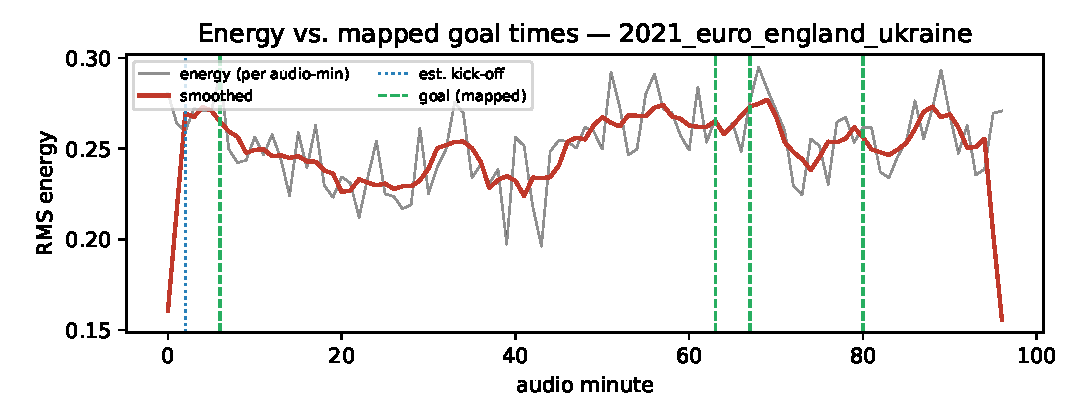
\includegraphics[width=0.82\linewidth]{figures/prosody_alignment.pdf}
\caption{Per-audio-minute RMS energy for the 2021 England--Ukraine match (England won 4--0). Dotted line: goal-independent kick-off estimate; dashed lines: the four goals mapped through that estimate plus a fixed half-time gap. Goals cluster on local energy maxima, but the visible imperfection of the mapping is exactly the alignment bottleneck quantified in Section~\ref{sec:prosody}.}
\label{fig:prosody}
\end{figure}

% ============================================================
\section{Qualitative Analysis}
\label{sec:qualitative}

The faithfulness probes of Section~\ref{sec:faith} quantify \emph{that} models hallucinate; this section shows \emph{what} the hallucinations look like. We inspected predictions for all 9 test matches; Table~\ref{tab:samples} shows sample outputs for the 2001 FA Cup Final (Arsenal--Liverpool, true score 1--2 with Owen scoring twice late on against Ljungberg's opener).

\begin{table}[h]
\centering\small
\begin{tabular}{p{0.18\linewidth}p{0.72\linewidth}}
\toprule
\textbf{Model} & \textbf{Output (first 250 chars)} \\
\midrule
\texttt{flan\_chunk\_zero} & ``Mark Warburton and Jamie Vardy contributed to BBC Radio 5 live coverage of Arsenal drew 1--1 at Anfield on Saturday.'' \\
\texttt{led\_long\_zero}   & ``\dots ope, and now to his right, the ball is going to the right side of the penalty area, it's going to be difficult to get the ball back to the left side\dots'' \\
\texttt{finetuned\_bart}   & ``Tour of the World Economic Forum (TEA) aims to showcase the benefits and potential benefits of travelling around the globe in a variety of ways. The event will provide a chance for people to experience\dots'' \\
\texttt{finetuned\_led}    & ``Liverpool 1--0 Arsenal. 2023--24 UEFA Cup Final, Millennium Stadium, Cardiff, UK -- 24 May 2021. Liverpool took the lead in the 11th minute when Mohamed Salah curled a low shot into the top corner from close range after a we\dots'' \\
\bottomrule
\end{tabular}
\caption{Sample outputs on the 2001 FA Cup Final test instance.}
\label{tab:samples}
\end{table}

\paragraph{What we observe.}
\begin{itemize}[leftmargin=*,itemsep=2pt,topsep=2pt]
\item \textbf{FLAN-T5} produces short, stylistically wrong (radio-broadcast snippet) and factually wrong content. With few-shot prompting, it copies the example target verbatim rather than summarising, a classic template-completion failure.
\item \textbf{LED prompting} generates fragments of mid-commentary text that mimic the input style rather than summarising it. The model is not pre-trained for summarisation and out-of-the-box behaves as a continuation language model.
\item \textbf{Fine-tuned BART} derails off-domain entirely on this instance --- its single both-teams failure in Table~\ref{tab:faith}. On the other eight test matches it produces exactly the structured, fluent match-report register the references teach, while \emph{inventing} the facts: for the 2019 UCL final it reports ``\emph{Liverpool 2--2 Tottenham Hotspur (Liverpool win 4--3 on penalties)}'' at Wembley --- the real final ended 2--0 to Liverpool in Madrid, with no shootout.
\item \textbf{Fine-tuned LED} similarly produces fluent match-report prose while inventing the factual frame: it reports the wrong score (1--0 actually 1--2), misdates the match to 2021, mislabels it a ``2023--24 UEFA Cup Final'' (actually the 2001 FA Cup Final), and populates the report with anachronistic scorers (Mohamed Salah, Mohamed Elneny) who took no part in a 2001 fixture. It does land the correct venue --- the Millennium Stadium in Cardiff, where the 2001 final was indeed played --- the lone grounded detail amid an otherwise fabricated report.
\end{itemize}

In short: both fine-tuned models have learned the \emph{format} of a match report, and neither has learned \emph{factual fidelity} --- the mechanism behind the metric decoupling quantified in Sections~\ref{sec:faith} and~\ref{sec:semantic}.

% ============================================================
\section{Engineering History}
\label{sec:engineering}

The path to the results in Section~\ref{sec:results} included several costly silent failures. We document them because each has independent reproducibility value and because the engineering choices behind the final numbers are not visible in the metrics.

\subsection{LED fine-tuning: five silent failures}
Early attempts to fine-tune LED failed silently: in two runs evaluation ROUGE-L dropped to zero by epoch~3 even as evaluation \emph{loss} continued to decrease, and a third crashed during evaluation at epoch~6. Table~\ref{tab:bugs} summarises the five defects that had to be found and fixed --- three hyperparameter changes were tried and failed first, because none of the failures was a modelling problem.

\begin{table}[h]
\centering\small
\begin{tabular}{p{0.30\linewidth}p{0.28\linewidth}p{0.32\linewidth}}
\toprule
\textbf{Bug} & \textbf{Symptom} & \textbf{Fix} \\
\midrule
Transcripts pre-truncated to 8192 tokens \emph{before} the random-window sampler & Random offset always 0: model saw only the first $\sim$8 min of every match & Truncate inside the sampler, after the offset is drawn \\
Collapse to immediate \texttt{<s></s>} under cross-entropy & ROUGE-L $=0$ while \texttt{eval\_loss} kept improving & \texttt{min\_length=80} at evaluation exposes (not masks) the collapse \\
$-100$ sentinels in \emph{prediction} tensors & \texttt{OverflowError} in \texttt{batch\_decode} (negative $\to$ \texttt{u32}) & Clip negatives to \texttt{pad\_id} before decoding \\
Crash before \texttt{save\_model()} & Inference 404 on \texttt{model.safetensors} & Fall back to latest \texttt{checkpoint-N/} \\
Kaggle CLI truncates non-ASCII filenames on Windows & Good files silently overwritten by 0-byte placeholders & Python API + \texttt{PYTHONIOENCODING=utf-8}, manual pagination \\
\bottomrule
\end{tabular}
\caption{The five silent failures encountered during LED fine-tuning.}
\label{tab:bugs}
\end{table}

After all five fixes, LED training ran cleanly through 11 epochs on the poisoned dataset (run~3): evaluation loss fell monotonically while validation ROUGE-L rose from 0.107 to a peak of 0.172 at epoch~9. We subsequently retrained from scratch on the clean dataset (run~5, Figure~\ref{fig:led_curve}): training ran 14 epochs, with validation ROUGE-L peaking at 0.270 at epoch~12 (early stopping with patience~2), and reaching a clean-trained test ROUGE-L of 0.248 (Table~\ref{tab:main}) --- at $n=9$, statistically indistinguishable from fine-tuned BART and nominally ahead on both ROUGE-L and BERTScore.

\begin{figure}[h]
\centering
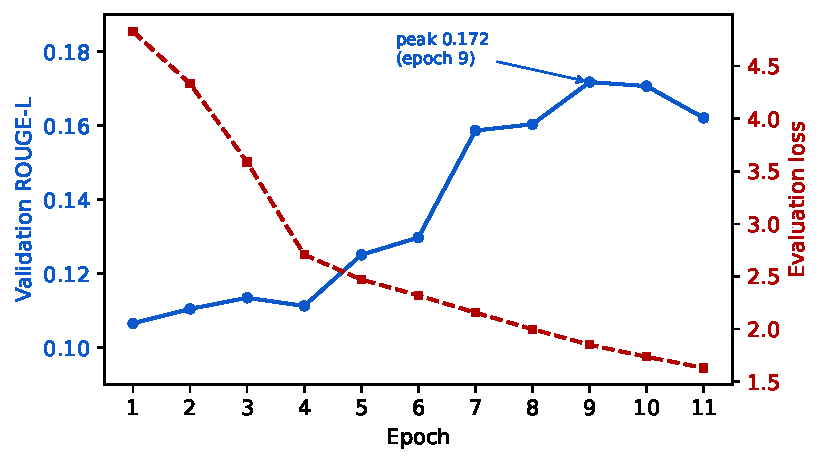
\includegraphics[width=0.72\linewidth]{figures/led_training_curve.pdf}
\caption{LED fine-tuning run~5 (clean dataset). Validation ROUGE-L (blue, left axis) peaks at 0.270 at epoch~12; evaluation loss (red, right axis) decreases monotonically. The selected checkpoint (epoch~12) yields test ROUGE-L~$=$~0.248. Contrast with pre-fix run~3 (11 epochs, peak 0.172), where identical-looking loss curves masked a ROUGE collapse caused by the empty-reference dataset bug.}
\label{fig:led_curve}
\end{figure}

\subsection{Empty-reference dataset incident}
The single most impactful fix in the project came from \emph{inspecting the raw inputs}. Investigating why generated summaries hallucinated obvious facts despite ROUGE-L $\sim$0.14, we opened a reference file and found it was 0~bytes; an audit showed 33\% of training references (26/80), 30\% of validation references (3/10), and 44\% of test references (4/9) were empty --- a stale local dataset copy. The damage was twofold: ROUGE against an empty reference is exactly 0, deflating every test average by $\sim$1.8$\times$; and a third of training pairs were $(\text{transcript}, \text{``''})$, teaching the models to emit nothing --- the actual root cause of LED's collapse-to-EOS that no hyperparameter change had touched. After pulling the repaired dataset and re-running, the measured improvements (1.7--1.9$\times$ across conditions, Table~\ref{tab:empty}) closely bracket the predicted 1.8$\times$, confirming the empty targets accounted for nearly all of the previous underperformance.

\begin{table}[h]
\centering\small
\begin{tabular}{lrrr}
\toprule
\textbf{Condition} & \textbf{Before fix} & \textbf{After fix} & $\boldsymbol{\Delta}$ \\
\midrule
finetuned\_bart   & 0.1361 & 0.2476 & +82\% \\
led\_long\_zero   & 0.0825 & 0.1599 & +94\% \\
flan\_chunk\_zero & 0.0413 & 0.0700 & +69\% \\
\bottomrule
\end{tabular}
\caption{ROUGE-L before and after the empty-reference fix.}
\label{tab:empty}
\end{table}

\subsection{Naive truncated-input BART fine-tuning}
The first BART fine-tune trained on \texttt{(transcript[:1024], reference)} pairs and reached ROUGE-L $= 0.127$. Replacing the input with the concatenation of pre-trained per-chunk summaries --- matching the inference-time pipeline --- raised ROUGE-L to $0.136$ on the broken dataset and to $0.248$ after the dataset fix. The combined train/inference distribution match plus two-phase optimisation accounts for the entire gap between naive and final fine-tuned BART.

% ============================================================
\section{Limitations}
\label{sec:limitations}

\paragraph{Small test set.} With $n = 9$ matches, only large differences are resolvable. The bootstrap analysis (Table~\ref{tab:main}) makes this concrete: fine-tuning vs.\ every prompting condition is significant, but the fine-tuned LED--BART gap ($-0.0004$, CI $[-0.042, +0.035]$) is not, and BART's CI alone spans $[0.208, 0.283]$. Rankings within $\pm 0.04$ ROUGE-L of each other should not be over-read.

\paragraph{The split under-serves small strata.} Our stratifier (\texttt{src/data/splits.py}) groups matches into four coarse competition buckets and then assigns splits round-robin across buckets, taking the first element of each in turn. For buckets larger than the test size this approximates proportional allocation, but for a bucket smaller than the number of splits it does the opposite of stratification: both FA Cup matches --- the entire bucket --- landed in the test set, leaving \emph{zero} FA Cup matches in training. Two of nine test matches (22\%) therefore come from a competition the fine-tuned models never saw, and both are conspicuous failures: the 1983 final is the oldest and noisiest audio in the corpus, and the 2001 final is the single instance on which fine-tuned BART derails entirely off-domain (Section~\ref{sec:qualitative}) and its only both-teams miss in Table~\ref{tab:faith}. We report the numbers as measured and did not re-split, since the split was fixed before any model was trained and changing it after seeing results would be a worse methodological error. The effect is not symmetric across the two fine-tuned models, and the asymmetry matters for how Observation~2 should be read. On the two FA Cup matches, chunk-merger BART averages ROUGE-L 0.189 against 0.264 on the other seven --- they are its two weakest instances and the main source of the wide CI in Table~\ref{tab:main} (per-match SD $0.062$, falling to $0.047$ when they are excluded) --- whereas long-context LED averages 0.255 on them against 0.246 elsewhere, i.e.\ marginally \emph{above} its own mean. Restricted to the seven in-distribution matches the nominal ordering of the two fine-tuned models therefore reverses (BART $0.264$ vs.\ LED $0.246$). At $n = 7$ that is far too little evidence to claim BART is really ahead, and we do not claim it. The point is the more cautious one: the 0.0004 separating the two models in Table~\ref{tab:main} is not only small relative to its confidence interval, it also moves under a known artefact of the split. That is a further reason to read them as joint first rather than ranked. A stratifier that allocates proportionally within each bucket --- or that merges buckets below a minimum size --- would remove the artefact.

\paragraph{Faithfulness is measured only coarsely.} Section~\ref{sec:faith} quantifies hallucination for scorelines, scorer recall, and named-entity precision, but the probes remain rule-based and schema-bound: named-entity precision is estimated from spaCy \texttt{PERSON} tags against the reference's people --- reliable only for the two fine-tuned models, which name enough entities to escape small-denominator noise --- and facts outside the score/scorer/person schema (dates, stadiums, competitions) remain unmeasured. A full NER-precision measure over all entity types and a human faithfulness rating would complete the picture.

\paragraph{GPT-4 references introduce evaluation bias.} References in Section~\ref{sec:gpt_targets} were generated by search-enabled GPT-4 (ChatGPT web) from match identifiers, not written from the transcript. Web retrieval grounds their facts in published match reports --- BBC sources were verified per match --- so outright factual errors are less likely than with purely parametric generation --- but the references still describe the match as the written press covered it, not as the radio commentary presented it, and they exhibit a stylistic homogeneity that surface metrics reward. They are also not exactly reproducible, since the underlying search results drift over time. Our reported scores therefore measure agreement with a GPT-4-distilled synthesis of web coverage, not agreement with a human gold standard paired to the input.

\paragraph{NLI support rates are conservative and coarse.} The NLI measure inherits Whisper's transcription noise in its premises, retrieves only three 60-word windows per sentence (support located elsewhere in a 25\,000-word transcript is missed), and is penalised by the register gap between summary-level assertions and fragmented spoken commentary. Absolute rates are therefore lower bounds and should not be read as ``x\% of content is true''; only the cross-condition comparison is meaningful. The register-insensitive score/scorer probes partially compensate, but a human faithfulness evaluation on the 9 test matches remains the gold-standard check we did not perform.

\paragraph{Whisper noise depresses surface metrics, but is not the faithfulness floor.} Systematic player-name errors (``Bergkamp'' $\to$ ``Burgkamp'') propagate into model outputs and cost surface overlap against correctly-spelled references, and the pre-2000 audio is markedly noisier than recent recordings, contributing to per-match variance. It does not, however, explain the faithfulness results: every one of the 22 reference scorers in the test set is present in the transcripts the models read (Section~\ref{sec:faith}), so the information the models fail to extract was never lost in transcription.

\paragraph{Reference-based metrics are format-saturated.} Section~\ref{sec:null} shows 84\% of our best ROUGE-L is attainable with no correct match content, so every gap here should be read against a null floor of $\approx 0.21$ rather than against zero. The caution applies more sharply to BERTScore, which we report raw rather than baseline-rescaled: its values are compressed into a narrow band (0.79--0.87 across all conditions) and support only an ordering --- the 0.009 between the two fine-tuned models is not interpretable, and we do not claim it.

\paragraph{$N = 80$ is the binding training constraint.} Both fine-tuned models likely overfit. The validation-to-test gap (BART $0.21 \to 0.14$ on the broken set; $0.31 \to 0.25$ on the clean set, where clean validation ROUGE-L peaks at 0.308) supports this. More data is the highest-leverage improvement.

% ============================================================
\section{Conclusions}

We built an end-to-end pipeline for summarising long football radio commentaries on a custom 99-match dataset, comparing two input strategies (chunk-and-aggregate vs.\ long-context LED) and two learning paradigms (prompting vs.\ fine-tuning) across three model families (FLAN-T5, BART, LED). Four findings stand out:

\begin{enumerate}[leftmargin=*,itemsep=2pt,topsep=2pt]
\item Fine-tuning BART as the merge step of a chunk-aggregate pipeline gives a $+55\%$ relative ROUGE-L improvement over the strongest prompting baseline ($+69\%$ over the same pre-trained model under the same pipeline), and the paired bootstrap confirms the fine-tuning-vs-prompting gap is significant for every prompting condition. Null baselines put that in proportion: the prompting baselines score below a content-free template, and the margin surviving a format-matched control is $+0.040$ ROUGE-L ($[+0.022, +0.059]$) --- significant, but a fifth of the headline.
\item Among prompting baselines, long-context (LED-16384) dominates chunk-aggregate when no fine-tuning is applied; among fine-tuned models, long-context LED is nominally ahead of chunk-aggregate BART (0.2480 vs.\ 0.2476) but the difference is within noise at $n=9$ --- the honest conclusion is that both fine-tuned pipelines work and neither separates from the other at this data scale.
\item In both chunk-aggregate families, zero-shot prompts outperform few-shot and chain-of-thought variants --- consistent with prompt-budget pressure --- and long-context LED is insensitive to the prompt styles tested, consistent with its non-instruction-tuned pre-training. (LED few-shot fell back to zero-shot through an implementation gap and remains untested.)
\item Reference similarity and source grounding come apart at the top of the leaderboard. Across the full condition range the two track each other weakly and positively ($\rho = +0.4$ to $+0.6$), but among the leaders the signal disappears: fine-tuned LED leads on every reference-based metric (ROUGE-L, BERTScore) yet achieves only 2/9 correct scorelines and 2\% NLI-entailed sentences, and fine-tuned BART goes further --- \textbf{0 of 9} correct scores and \textbf{zero} NLI-supported sentences while ranking second on ROUGE and BERTScore. A metric that discriminates everywhere except among the candidates you are choosing between is not usable for model selection on this task. The best-grounded condition is the transcript-copying prompted LED that both fine-tuned models dominate on reference metrics (34\% NLI support). Surface metrics reward format imitation, not factual fidelity, and the null baselines quantify how much: 84\% of our best ROUGE-L needs no correct match content. Nor is this an information-availability failure --- all 22 reference scorers appear in the transcripts the models read.
\end{enumerate}

The largest single improvement in the project came not from a model change but from \emph{detecting and fixing a 33\% empty-reference rate in the training data}, which had been silently teaching all models to emit empty strings. Equally instructive, the faithfulness probes show that fine-tuned models learn the surface form of a match report while inventing its facts. Reliable football-match summarisation requires optimising a faithfulness signal --- not merely measuring one, as we do here; designing that training signal is the natural next step beyond this work.

% ============================================================
\bibliographystyle{plainnat}
{\small\bibliography{refs}}

% Fallback if natbib not desired: uncomment the following and remove \bibliography above.
% \begin{thebibliography}{20}
%   \bibitem[Lewis et al.(2020)]{lewis2020bart} ...
% \end{thebibliography}

\end{document}
